\newgeometry{top=1cm, bottom=2cm}
\section{Lineare Abbildungen}
\begin{figure}[h!]
    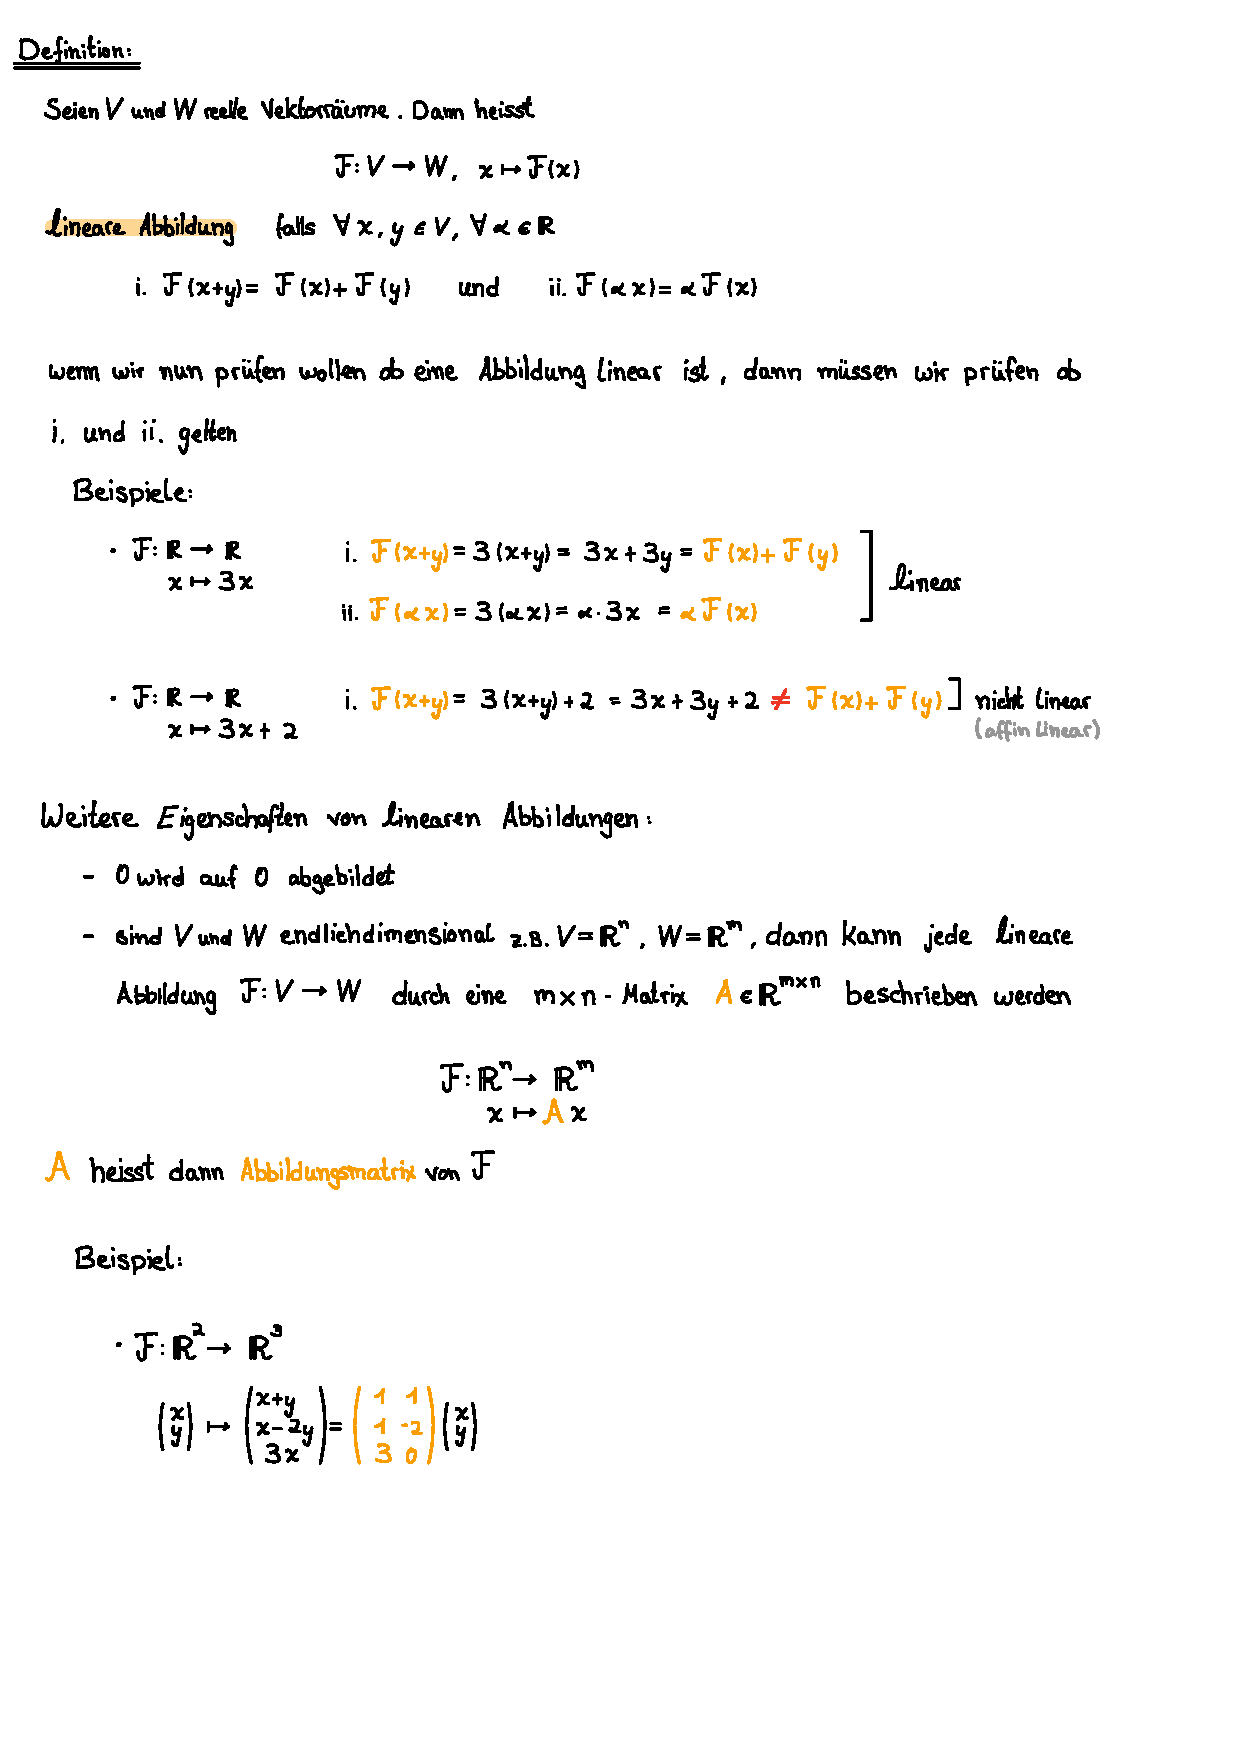
\includegraphics[page=1, scale=0.842]{pdf/05_Lineare_Abbildungen.pdf}
\end{figure}
\newpage
\includepdf[pages={2-}, 
            pagecommand={\thispagestyle{plain}}, 
            scale=0.95]{pdf/05_Lineare_Abbildungen.pdf}

\newgeometry{top=2.5cm, bottom=2cm}
\subsection{Beispielaufgaben} %Übung 01
\vspace{1cm}
\subsubsection{} %serie 06
Sei
\[
A = \begin{pmatrix}
2 & 1 & -1 & 2 \\
1 & 0 & -1 & 0 \\
3 & 1 & -2 & 2 \\
\end{pmatrix}.
\]
Bestimmen Sie eine Basis für das Bild und den Kern von $A$. \\

\noindent \textbf{Lösung:}
\vspace{5cm}

\subsubsection{} %Prüfiung S.12
Sei $\mathcal{P}_2$ der Vektorraum der Polynome vom Grad $\leq 2$ mit der Basis $\mathcal{B} = \{1,x,x^2\}$. Sei
\[\begin{aligned}
\mathcal{L}: \; \mathcal{P}_2 &\rightarrow \mathcal{P}_2 \\
p(x) &\mapsto p''(x)+4p'(x)+3p(x)
\end{aligned}\] \\
Bestimmen Sie die Darstellungsmatrix von $\mathcal{L}$ bezüglich der Basis $\mathcal{B}$.\\

\noindent \textbf{Lösung:}

\newpage
\subsubsection{}
Geben seinen die Abbildungen
\begin{enumerate}[label=\alph*)]
    \item $\mathcal{F}: \mathbb{R}^2 \rightarrow \mathbb{R}^2,\; (x_1,x_2)^\top \mapsto (2x_1+x_2,x_1)^\top $
    \item $\mathcal{G}: \mathcal{C} ([x_0,x_1], \mathbb{R}) \rightarrow \mathbb{R},\; g(x) \mapsto \int_{x_0}^{x_1} g(x) \,dx$
\end{enumerate}
Prüfe ob die Abbildungen $\mathcal{F,G}$ linear sind.\\

\noindent \textit{Tipp}: $\mathcal{C} ([x_0,x_1], \mathbb{R})$ beschreibt alle stetigen Funktionen auf dem Intervall $[x_0,x_1]$. \\

\noindent \textbf{Lösung:}

% \newpage
% \subsubsection{}
% Sei $V = \mathcal{P}_2$ und $W = \mathcal{P}_1$. Wobei V durch die Basis $\mathcal{B} = (1,x,x^2)$ und $W$ durch die Basis $\mathcal{C} = (1,x)$ beschrieben werden kann. sei ausserdem
% \[\begin{aligned}
% \mathcal{F}: \; V &\rightarrow W \\
% p(x) &\mapsto p'(x)+p''(x)
% \end{aligned}\]
% Bestimme die Abbildungsmatrix $A$ der Abbildung $\mathcal{F}$. \\

% \noindent \textbf{Lösung:}

\newpage
\subsubsection{} %Serie 06
Gegeben Sei der Vektorraum $V = \mathbb{R}^3$ mit der Standardbasis $\mathcal{B}$. Die Matrix
\[
A = \begin{pmatrix}
-\frac{5}{6} & \frac{1}{6} & \frac{1}{3} \\
\frac{1}{6}  & -\frac{5}{6} & \frac{1}{3} \\
\frac{1}{3} & \frac{1}{3} & -\frac{1}{3} \\
\end{pmatrix}.
\]
definiert eine lineare Abbildung von $V$ nach $V$.
\begin{enumerate}[label=\alph*)]
    \item Durch eine Wahl der neuen Basis
           \[ \mathcal{B}' = \Biggl\{ 
                                \begin{pmatrix}
                                2\\
                                0\\
                                -1\\
                                \end{pmatrix},
                                \begin{pmatrix}
                                -1\\
                                1\\
                                0\\
                                \end{pmatrix},
                                \begin{pmatrix}
                                1\\
                                1\\
                                2\\
                                \end{pmatrix}
                                \Biggr\}.
                                \]
            werden neue Koordianten eingeführt. Bestimmen Sie die Übergangsmatrix $T$ von $\mathcal{B}$ nach $\mathcal{B}'$.
            \item Durch welche Matrix $B$ wird die lineare Abbildung in den neuen Koordinaten $\mathcal{B}'$ beschrieben?
\end{enumerate}

\newpage
\subsubsection{} %Zardini S.84
Betrachten Sie die Abbildung $\mathcal{F}: \mathbb{R}^3 \rightarrow \mathbb{R}^3$ gegeben durch
\[
\begin{pmatrix}
x\\
y\\
z\\
\end{pmatrix} \mapsto
\begin{pmatrix}
7x+5y-8z\\
5x+3y-4z\\
-x-3y+8z\\
\end{pmatrix}
\]
\begin{enumerate}[label=\alph*)]
    \item Geben Sie die Darstellungsmatrix von $\mathcal{F}$ bezüglich der Standardbasis $\mathcal{E} = \{e_1,e_2,e_3\}$ von $\mathbb{R}^3$ an.
    \item Gegeben sei die Basis $\mathcal{B} = \{b_1 := e_1,\; b_2 :=e_1+e_2,\; b_3 := e_2+e_3 \}$ von $\mathbb{R}^3$. Finden Sie die Übergangsmatrix $T$ von $\mathcal{B}$ nach $\mathcal{E}$ und ihre Inverse $T^{-1}$.
    \item Berechnen Sie die Darstellungsmatrix von $\mathcal{F}$ bezüglich $\mathcal{B}$ unter Verwendung der Übergangsmatrix $T$ und ihrer Inversen.
    \item Bestimmen Sie eine Basis des Kerns von $\mathcal{F}$ und eine Basis des Bildes von $\mathcal{F}$. Geben Sie ausserdem die jeweiligen Dimensionen an.
\end{enumerate}

\noindent \textbf{Lösung:}